\chapter{无人机编队整体控制逻辑、仿真环境以及硬件选型}
\label{chap:hardware}
本章主要介绍无人机编队的编队控制算法之外的系统组成部分;之后介绍无人机编队的整体的控制的实现逻辑,之后将介绍无人机编队的动力学仿真环境的搭建。
最后将介绍本次设计之中所用到的无人机型号,自动驾驶仪硬件以及姿态自动驾驶仪内环基本控制逻辑。
\section{无人机软硬件环境选配}
本文所设计的编队控制器是以开源自动驾驶仪$PX4$的内环为基础的,自动驾驶仪内环的作用是追踪来自位置环的无人机期望姿态;
算法所运行的软件环境是$ROS$(Robot Operating System)。$ROS$是一个适用于机器人的开源操作系统。
它提供了操作系统应有的服务,包括硬件抽象,底层设备控制,常用函数实现,进程间消息传递,以及包管理。
它也提供用于获取、编译、编写、和跨计算机运行代码所需的工具和库函数。本次使用的应用程序接口,是$ROS$下的$mavros$功能包,
本功能包的作用是:将来自自动驾驶仪的无人机状态数据由$mavlink$通信协议转换为$ROS$的进程间的通讯的协议;
将来自编队控制器的姿态驾驶仪内环的期望姿态角以及期望油门值按照$mavlink$的协议进行编码,从而起到沟通编队
控制器以及姿态驾驶仪内环的桥梁作用。编队控制算法运行在具有$ROS$环境的上位机(HOST COMPUTER)中,
稳定内环运行在下位机(Pixhawk)之中。整体的软件硬件选配关系如下图所示:
\begin{figure}[H]
    \centering
    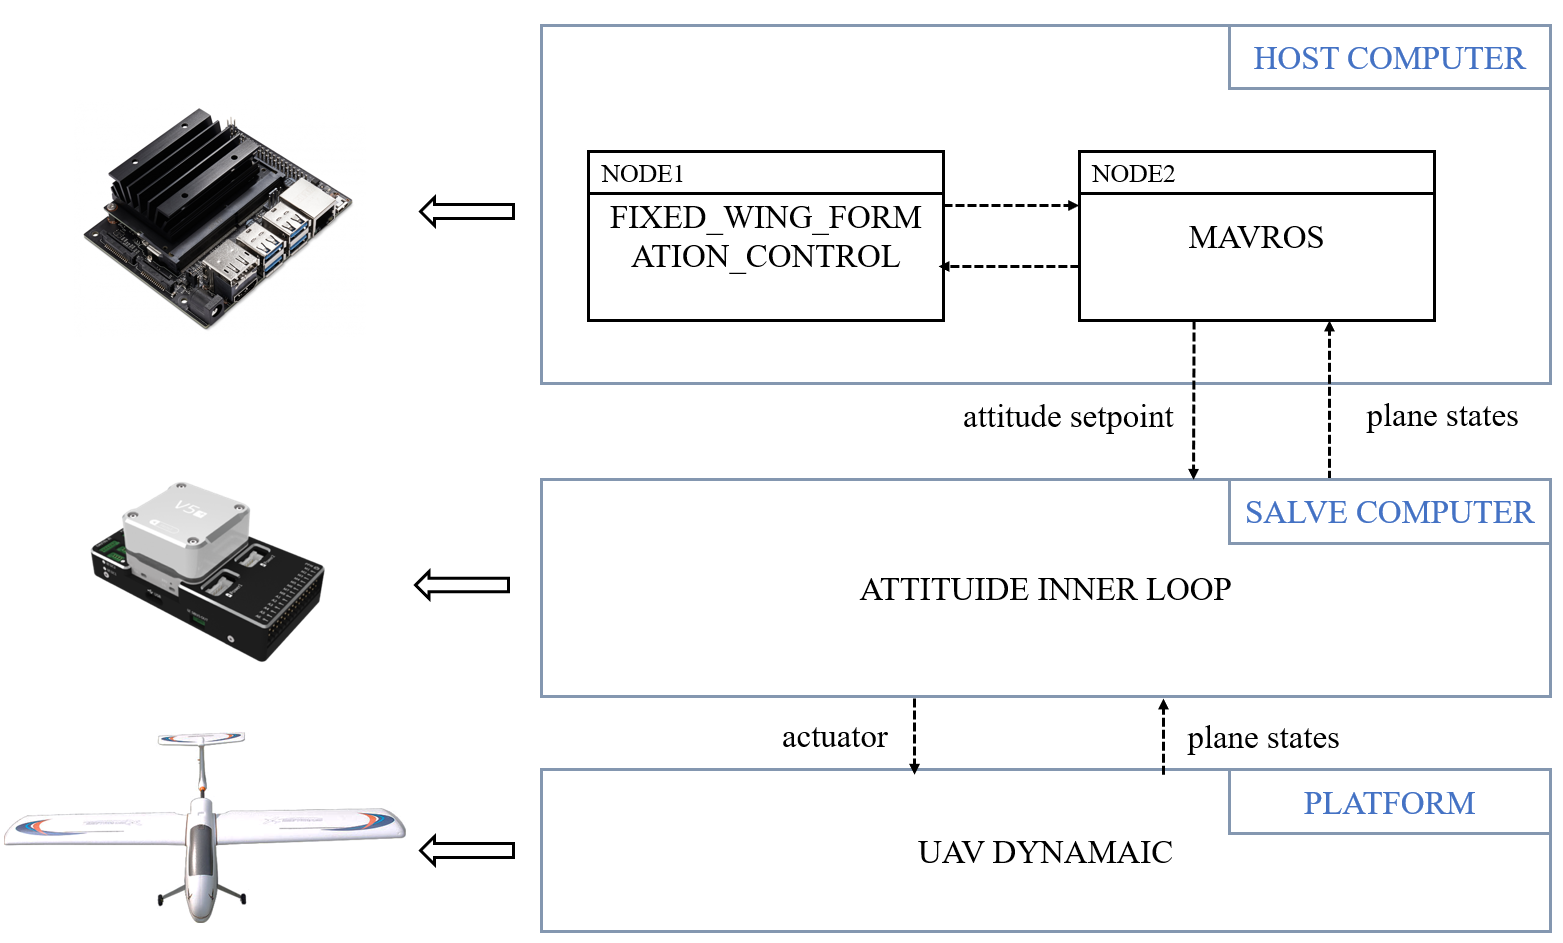
\includegraphics[width=1\textwidth]{figures/c4/c4-soft-hard.png}
    \caption{硬件软件选配关系}\label{fig:c4-soft-hard.png}
\end{figure}
\section{无人机编队动力学仿真环境}
所谓无人机动力学仿真环境,是在考虑无人机的空气动力的作用基础基础之上搭建的仿真环境,相较于控制器的数学仿真,此种仿真环境考虑了
无人机作为一个实际的被控系统而存在的过渡过程,不确定性以及扰动因素,将更加符合无人机飞行时的实际状态。
本次动力学仿真的搭建,是基于$Gazebo$仿真环境的。
\section{无人机编队硬件选型}
本次毕业设计之中所涉及的编队控制器的自动驾驶仪部分为开源硬件$Pixhawk$:
